\solutionset

\begin{enumerate}

\item \textbf{HII Region Trapping.}

\begin{enumerate}

\item The density profile of the accretion flow is given implicitly by
\begin{displaymath}
\dot{M}_* = 4\pi r^2 \rho v_{\rm ff},
\end{displaymath}
where $v_{\rm ff} = \sqrt{2 G M_*/r}$. Thus we have
\begin{displaymath}
\rho = \frac{\dot{M}_*}{4\pi \sqrt{2G M_*}} r^{-3/2}.
\end{displaymath}
Recombinations happen in the region between $R_*$ and $r_i$. The recombination rate per unit volume is $\alpha_B n_e n_p = 1.1 \alpha_B (\rho/\mu_{\rm H})^2$, where $\mu_{\rm H} =2.3\times 10^{-24}$ g is the mass per H nucleus assuming standard composition. Thus the total recombination rate within the ionized volume is
\begin{eqnarray*}
\Gamma & = & \int_{R_*}^{r_i} 4\pi r^2 (1.1\alpha_B) \left(\frac{\dot{M}_*}{4\pi \mu_{\rm H} \sqrt{2G M_*}} r^{-3/2}\right)^2 \, dr \\
& = & \frac{1.1\alpha_B \dot{M}_*^2}{8\pi \mu_{\rm H}^2 G M_*} \ln \frac{r_i}{R_*}.
\end{eqnarray*}
Since this must equal the ionizing photon production rate ($\Gamma = S$), we can solve for $r_i$:
\begin{displaymath}
r_i = R_* \exp\left(\frac{8\pi \mu_{\rm H}^2 G M_* S}{1.1 \alpha_B \dot{M}_*^2}\right).
\end{displaymath}
The condition that $r_i \gg R_*$ is satisfied if the term inside parentheses is $\gtrsim 1$, which in turn requires
\begin{displaymath}
\dot{M}_* \lesssim \left(\frac{8\pi \mu_{\rm H}^2 G M_* S}{1.1 \alpha_B}\right)^{1/2}.
\end{displaymath}
Plugging in the given values $M_* = 30$ $\msun$ and $S=10^{49}$ s$^{-1}$, we obtain $\dot{M}_* \lesssim 7\times 10^{-5}$ $\msun$ yr$^{-1}$. This is lower (though not by a huge amount) than the typical accretion rates inferred for massive stars.

\item The escape velocity at a distance $r$ from the star is $v_{\rm esc} = \sqrt{2 G M_*/r}$. Thus the condition that $v_{\rm esc} < c_i$ at $r_i$ implies that
\begin{displaymath}
\frac{2 G M_*}{c_i^2} <  r_i = R_* \exp\left(\frac{8\pi \mu_{\rm H}^2 G M_* S}{1.1 \alpha_B \dot{M}_*^2}\right).
\end{displaymath}
Solving for $\dot{M}_*$, we find
\begin{displaymath}
\dot{M}_* > \left[\frac{8\pi \mu_{\rm H}^2 G M_* S}{2.2\alpha_B \ln(v_{\rm esc,*}/c_i)}\right]^{1/2},
\end{displaymath}
where $v_{\rm esc,*} = \sqrt{2 G M_*/R_*}$ is the escape speed from the stellar surface. Using $R_*=7.7$ $\rsun$ (the radius of a 30 $\msun$ ZAMS star) and plugging in the other input values gives $\dot{M}_*>2.2\times 10^{-5}$ $\msun$.

\end{enumerate}

\item \textbf{The Transition to Grain-Mediated H$_2$ Formation}

\begin{enumerate}

\item To calculate the rate of H$_2$ formation catalyzed by free electrons, we first calculate the rate of formation of H$^-$:
\begin{displaymath}
\gamma({\rm H}^{-}\,{\rm form.}) = k_{-} n_e n_{\rm H} = k_{-} x_{\rm C} Z n_{\rm H}^2,
\end{displaymath}
where $k_{-} = 1.1\times 10^{-16} T_2^{0.88}$ cm$^3$ s$^{-1}$ is the rate coefficient given in Chapter \ref{ch:first_stars}. Next we must calculate the fraction of H$^-$ ions formed that yield H$_2$. The H$^-$ can be destroyed either by photodetachment or by reacting with a neutral hydrogen to form H$_2$:
\begin{displaymath}
{\rm H}^{-} + {\rm H} \rightarrow {\rm H}_2 + e^{-}.
\end{displaymath}
The rate of the latter reaction is
\begin{displaymath}
\gamma({\rm H}^{-}\rightarrow{\rm H}_2) = k_2 n_{{\rm H}^-} n_{\rm H}
\end{displaymath}
with $k_2 = 1.3\times 10^{-9}$ cm$^3$ s$^{-1}$ (the value given in class). The rate of photodetachment is
\begin{displaymath}
\gamma({\rm H}^{-}\,{\rm photo.}) = \zeta_{\rm pd} n_{{\rm H}^-}
\end{displaymath}
with $\zeta_{\rm pd} = 2.4\times 10^{-7}$ s$^{-1}$ for the Milky Way radiation field, again as given in class. Thus the branching ratio for H$^{-}$ going to H$_2$ rather than being destroyed by photodetachment is
\begin{displaymath}
\Gamma({\rm H}^{-}\rightarrow{\rm H}_2) = \frac{\gamma({\rm H}^{-}\rightarrow{\rm H}_2)}{\gamma({\rm H}^{-}\rightarrow{\rm H}_2) + \gamma({\rm H}^{-}\,{\rm photo.})} = \frac{k_2 n_{\rm H}}{k_2 n_{\rm H}+\zeta_{\rm pd}}
\end{displaymath}
Putting this together, the rate of formation of H$_2$ via free electrons is
\begin{eqnarray*}
\gamma({\rm H}_2{\rm - gas}) & = & \gamma({\rm H}^{-}\,{\rm form.}) \Gamma({\rm H}^{-}\rightarrow{\rm H}_2) \\
& = & k_{-} x_{\rm C} Z  \left[1+ \zeta_{\rm pd}/(k_2 n_{\rm H})\right]^{-1} n_{\rm H}^2. 
\end{eqnarray*}
In comparison, the rate of H$_2$ formation on grain surfaces is simply
\begin{displaymath}
\gamma({\rm H}_2{\rm - grain}) = R n_{\rm H}^2 = R_{\odot} Z n_{\rm H}^2,
\end{displaymath}
where $R_{\odot} = 3\times 10^{-17}$ cm$^3$ s$^{-1}$ is the rate coefficient at Solar metallicity. Taking the ratio of these two, we have
\begin{eqnarray*}
\frac{\gamma({\rm H}_2{\rm - grain})}{\gamma({\rm H}_2{\rm - gas})} & = & \frac{R_{\odot} \left[1+ \zeta_{\rm pd}/(k_2 n_{\rm H})\right]}{k_{-} x_{\rm C}} \\
& = & 2700 T_2^{-0.88} \left[1+ \zeta_{\rm pd}/(k_2 n_{\rm H})\right].
\end{eqnarray*}
Thus even in the limit $n_{\rm H} \rightarrow \infty$, the rate of formation on grain surfaces exceeds that in the gas phase by $\sim 3$ orders of magnitude. At densities below $\zeta_{\rm pd}/k_2 = 185$ cm$^{-3}$, where photodetachment significantly inhibits H$_2$ formation via the H$^-$ channel, grain formation wins by an even larger factor.\\

\item For gas phase formation, this calculation is exactly the same as the previous part, with two minor differences. First, the factor $x_{\rm C} Z$ in the gas-phase formation rate is replaced by $x$, since how hydrogen rather than carbon is the dominant source of free electrons. Second, all the $n_{\rm H}$ factors become $(1-x) n_{\rm H}$, since only neutral hydrogen participates in the relevant reactions. Making these changes, the H$^-$ formation rate is
\begin{displaymath}
\gamma({\rm H}^{-}\,{\rm form.}) = k_{-} x (1-x) n_{\rm H}^2,
\end{displaymath}
and the H$^-$ to H$_2$ reaction rate is
\begin{displaymath}
\gamma({\rm H}^{-}\rightarrow{\rm H}_2) = k_2 (1-x) n_{{\rm H}^-} n_{\rm H}.
\end{displaymath}
The photodetachment rate is unchanged, so the branching ratio for H$^-$ going to H$_2$ becomes
\begin{displaymath}
\Gamma({\rm H}^{-}\rightarrow{\rm H}_2) = \frac{k_2 (1-x) n_{\rm H}}{k_2 (1-x) n_{\rm H}+\zeta_{\rm pd}},
\end{displaymath}
and the gas-phase H$_2$ formation rate is therefore
\begin{displaymath}
\gamma({\rm H}_2{\rm - gas}) = k_{-} x (1-x)  \left[1+ \zeta_{\rm pd}/(k_2 (1-x) n_{\rm H})\right]^{-1} n_{\rm H}^2. 
\end{displaymath}
The grain-mediated reaction rate becomes
\begin{displaymath}
\gamma({\rm H}_2{\rm - grain}) = R_{\odot} Z (1-x) n_{\rm H}^2.
\end{displaymath}
Notice that there is only one factor of $x$, because the reaction rate involves the collision of neutral hydrogen atoms with dust grains, and therefore depends on the density of gas times the density of grains. If the ionization fraction is $x$, the neutral hydrogen fraction is reduced by a factor $(1-x)$, but the grain abundance is unchanged. Setting the two rates equal, we have
\begin{displaymath}
k_{-} x \left[1+ \zeta_{\rm pd}/(k_2 (1-x) n_{\rm H})\right]^{-1} = R_{\odot} Z.
\end{displaymath}
This is a quadratic in $x$, and the solution is
\begin{displaymath}
x = \frac{1}{2}\left(1+k \pm \sqrt{1-2k + k^2 - 4 k/r_{\rm pd}}\right)
\end{displaymath}
\begin{marginfigure}
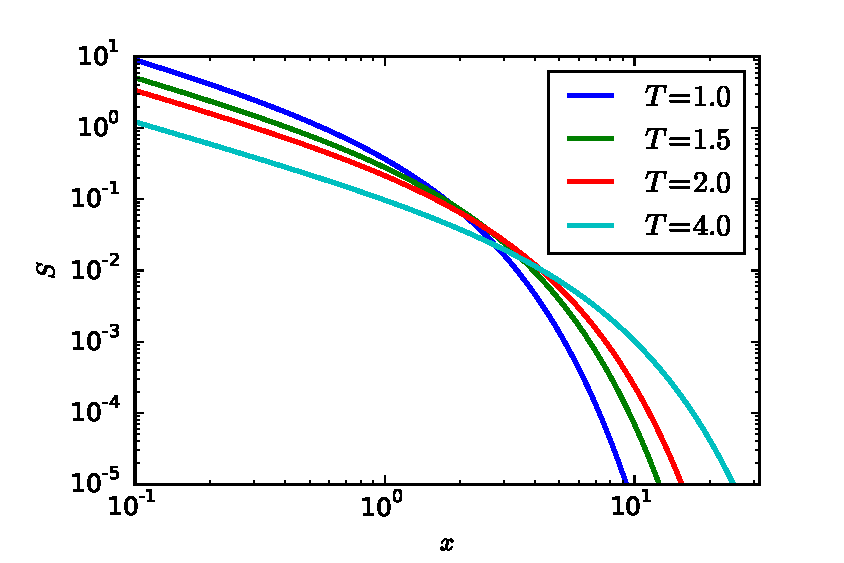
\includegraphics[width=\linewidth]{hw4sol1}
\caption[Solution to problem set~\thesolutionset, problem~\theenumi\theenumii]{
\label{fig:hw4sol1}
$x$ versus $Z$ for $n_{\rm H} = 1$, 10, and 100 cm$^{-3}$.
}
\end{marginfigure}
where $k = R_{\odot} Z/k_{-}\approx 0.27 T_2^{-0.88} Z$ is the ratio of the rate coefficients for H$_2$ formation on grains and H$^-$ formation in the gas phase, and $r_{\rm pd} = n_{\rm H} k_2 / \zeta_{\rm pd}$ is the ratio of the gas density to the critical density for H$_2$ photodetachment, $n_{\rm crit,pd} = \zeta_{\rm pd}/k_2\approx 185$ cm$^{-3}$. Note that both roots represent mathematically valid solutions, one at ionization fraction below 50\% and one at ionization fraction above 50\%. In practice, however, the low ionization fraction solution is the more physically-realistic one, since if the gas is highly ionized the temperature is unlikely to be low enough to allow formation of H$_2$. Figure \ref{fig:hw4sol1} shows the physically-realistic solution plotted for $n_{\rm H} = 1$, 10, and 100 cm$^{-3}$.

\item A solution ceases to exist when the metallicity is such that the quantity under the square root in the equation from the previous part goes to zero. Thus, grain-mediated H$_2$ formation must dominate whenever
\begin{displaymath}
1 - 2k + k^2 - 4 k r_{\rm pd}^{-1} < 0.
\end{displaymath}
Solving, this condition reduces to
\begin{displaymath}
k > 1 + \frac{2}{r_{\rm pd}} \left(1 - \sqrt{1+r_{\rm pd}}\right).
\end{displaymath}
(Note: there is another root to this equation, with a $+$ instead of a $-$ in front of the square root. However, one can easily verify that in the vicinity of this root $x>1$, which is obviously unphysical. Thus the $-$ root is the physically realistic one.) Rewriting this in terms of dimensional quantities, this is
\begin{marginfigure}
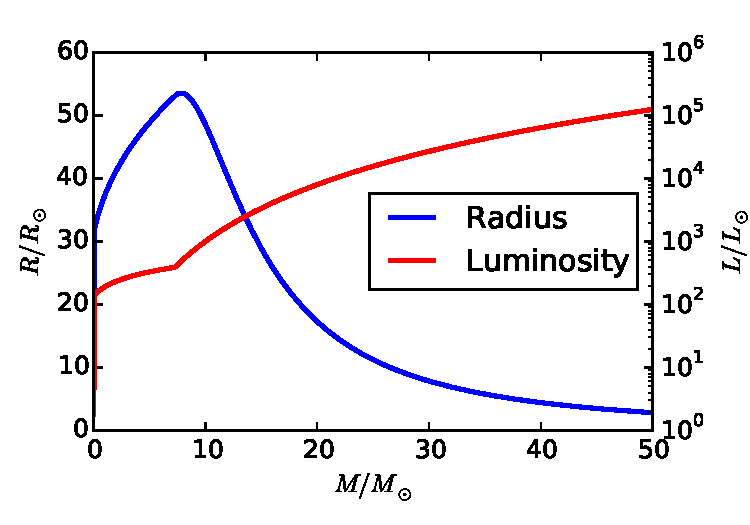
\includegraphics[width=\linewidth]{hw4sol2}
\caption[Solution to problem set~\thesolutionset, problem~\theenumi\theenumii]{
\label{fig:hw4sol2}
$Z$ versus $n_{\rm H}$ at $T=100$ K and $1000$ K.
}
\end{marginfigure}
\begin{displaymath}
Z > 0.27 T_2^{0.88} \left[1 + \frac{2 n_{\rm crit,pd}}{n_{\rm H}} \left(1 - \sqrt{1+\frac{n_{\rm H}}{n_{\rm crit,pd}}}\right)\right].
\end{displaymath}
Figure \ref{fig:hw4sol2} shows a plot of the minimum value of $Z$ versus density $n_{\rm H}$ at $T=100$ K and 1000 K.


\end{enumerate}

\item \textbf{Self-Similar Viscous Disks.}

\begin{enumerate}

\item First let us plug in the given form for $\nu$:
\begin{displaymath}
\frac{\partial\Sigma}{\partial t} = \frac{\nu_1}{\varpi_1} \frac{3}{\varpi} \frac{\partial}{\partial \varpi} \left[\varpi^{1/2} \frac{\partial}{\partial \varpi} \left(\Sigma \varpi^{3/2}\right)\right].
\end{displaymath}
Next, let's make the change of variables $\varpi = \varpi_1 x$. Note that this also implies that $\partial /\partial \varpi = (1/\varpi_1) \partial/\partial x$. With this change, we have
\begin{displaymath}
\frac{\partial\Sigma}{\partial t} = \frac{\nu_1}{\varpi_1^2} \frac{3}{x} \frac{\partial}{\partial x} \left[x^{1/2} \frac{\partial}{\partial x} \left(\Sigma x^{3/2}\right)\right].
\end{displaymath}
The third step is to make the change of variables $t = T t_s$, $\partial/\partial t = (1/t_s) \partial/\partial T$, then simplify:
\begin{eqnarray*}
\frac{3\nu_1}{\varpi_1^2} \frac{\partial\Sigma}{\partial T} & = & \frac{\nu_1}{\varpi_1^2} \frac{3}{x} \frac{\partial}{\partial x} \left[x^{1/2} \frac{\partial}{\partial x} \left(\Sigma x^{3/2}\right)\right] \\
\frac{\partial\Sigma}{\partial T} & = & \frac{1}{x} \frac{\partial}{\partial x} \left[x^{1/2} \frac{\partial}{\partial x} \left(\Sigma x^{3/2}\right)\right].
\end{eqnarray*}
The last step is to substitute in for $\Sigma$, which is trivial:
\begin{displaymath}
\frac{\partial S}{\partial T} = \frac{1}{x} \frac{\partial}{\partial x} \left[x^{1/2} \frac{\partial}{\partial x} \left(S x^{3/2}\right)\right].
\end{displaymath}
This is the non-dimensional equation we wanted.

\item We can show that the given form is a solution simply by plugging in the equivalent non-dimensional solution for $S$, which is
\begin{displaymath}
S = \frac{e^{-x/T}}{x T^{3/2}}.
\end{displaymath}
Plugging this into the two sides of the non-dimensional equation, we get
\begin{eqnarray*}
\frac{\partial S}{\partial T} & = & \left(\frac{2x - 3 T}{2 x T^{7/2}}\right) e^{-x/T} \\
\frac{1}{x} \frac{\partial}{\partial x} \left[x^{1/2} \frac{\partial}{\partial x} \left(S x^{3/2}\right)\right]
& = & 
\frac{1}{x} \frac{\partial}{\partial x} \left[\left(\frac{T-2x}{2 T^{5/2}}\right) e^{-x/T}\right] \\
& = & \left(\frac{2x - 3 T}{2 x T^{7/2}}\right) e^{-x/T}.
\end{eqnarray*}
Since the two sides match, this suffices to show that $S=e^{-x/T}/(x T^{3/2})$ is a solution. Since we have made no assumptions about the value of $\Sigma_1$ in this argument, we are free to choose its value to be whatever we want. In particular, if we choose $\Sigma_1 = C/3\pi \nu_1$, then we immediately obtain the solution
\begin{displaymath}
\Sigma = \left(\frac{C}{3\pi \nu_1}\right)\frac{1}{x T^{3/2}} e^{-x/T}.
\end{displaymath}

\item The disk mass is simply given by
\begin{eqnarray*}
M_d & = & \int_0^\infty 2\pi \varpi \Sigma \, d\varpi \\
& = & \varpi_1^2 \int_0^\infty 2\pi x \Sigma \, dx \\
& = & \left(\frac{2 C \varpi_1^2}{3 \nu_1}\right) \frac{1}{T^{3/2}} \int_0^\infty e^{-x/T} \, dx \\
& = & \frac{2 C \varpi_1^2}{3 \nu_1 T^{1/2}} \\
& = & 2 C t_s \left(\frac{t}{t_s}\right)^{-1/2}.
\end{eqnarray*}
The time rate of change of the disk mass is just
\begin{displaymath}
\dot{M}_d = -C \left(\frac{t}{t_s}\right)^{-3/2}.
\end{displaymath}
Looking at the equation, and noting that $C$ has units of mass per time, it is clear that $C$ controls the accretion rate of the disk onto the point mass in the center.

\begin{marginfigure}
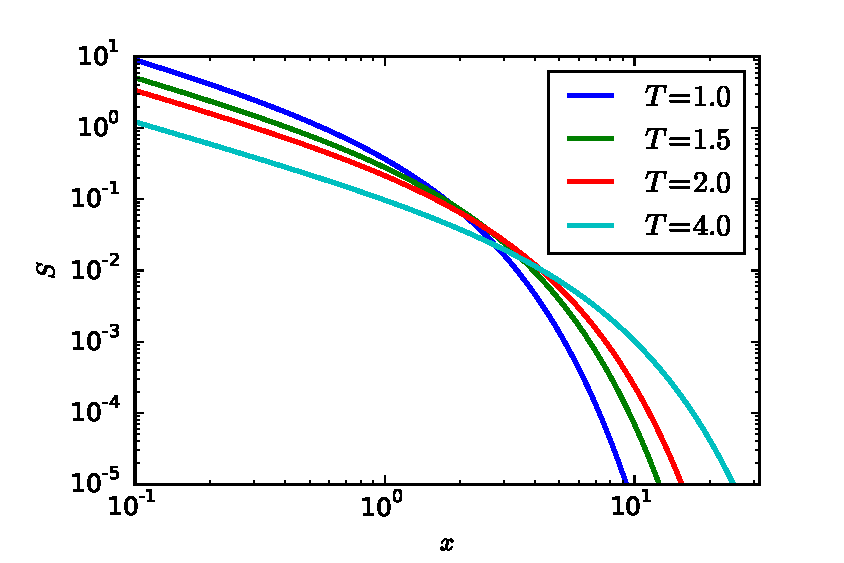
\includegraphics[width=\linewidth]{hw4sol3}
\caption[Solution to problem set~\thesolutionset, problem~\theenumi\theenumii]{
\label{fig:hw4sol3}
$S$ versus $x$ at dimensionless times $T=1, 1.5, 2$, and 4.
}
\end{marginfigure}
\item Figure \ref{fig:hw4sol3} shows the required plot. We see that the disk surface density profile follows $S\propto x^{-1}$ for $x<T$, and is exponentially truncated at $x>T$. We can think of the inner part as the ``main disk", and the outer part as the material pushed outward by viscosity in order to compensate for the angular momentum lost as other gas moves inwards. As time passes, the inner, main disk drains onto the star, and its surface density decreases. At the same time, the outer, exponentially truncated segment of the disk grows to larger and larger radii as more and more angular momentum is extracted from the inner disk.

\end{enumerate}

\item \textbf{A Simple T Tauri Disk Model.}

\begin{enumerate}

\item The disk interior is optically thick, so the vertical radiation flux $F$ is given by the diffusion approximation:
\begin{displaymath}
F = \frac{c}{3\kappa\rho} \frac{d}{dz} E = \frac{ca}{3\kappa\rho} \frac{d}{dz} (T^4) = \frac{4 \sigma}{3\kappa\rho}  \frac{d}{dz} (T^4)
\end{displaymath}
where $E$ is the radiation energy density and $T$ is the gas temperature. In thermal equilibrium the flux does not vary with $z$, so we can re-arrange this equation and integrate from the midplane at $z=0$ to the surface at $z=z_s$:
\begin{eqnarray*}
F \int_0^{z_s} \rho \, dz & = & \frac{4\sigma}{3\kappa} \int_{T_m}^{T_s} \frac{d}{dz} T^4 \, dz \\
F \frac{\Sigma}{2} & = & \frac{4\sigma}{3\kappa} \left(T_m^4 - T_s^4\right) \\
F & \approx & \frac{8\sigma}{3\kappa\Sigma} T_m^4,
\end{eqnarray*}
where the factor of 2 in the denominator on the LHS in the second step comes from the fact that $\Sigma$ is the column density of the entire disk, and we integrated over only half of it. In the third step we assumed that $T_m^4 \gg T_s^4$, which will be true for any optically thick disk. Note that this is the flux carried away from the disk midplane in both the $+z$ and $-z$ directions -- formally the flux changes direction discontinuously at $z=0$ in this simple model, so the total flux leaving the midplane is twice this value. If the disk radiates as a blackbody, the radiation flux per unit area leaving each side of the disk surface is $\sigma T_s^4$, and this must balance the flux that is transported upward through the disk by diffusion. Thus we have
\begin{displaymath}
\frac{8\sigma}{3\kappa\Sigma} T_m^4 \approx \sigma T_s^4,
\end{displaymath}
where the expressions on either side of the equality represent the fluxes in either the $+z$ or $-z$ directions either; the total fluxes are a factor of 2 greater, but the factors of 2 obviously cancel. Solving for $T_m$ gives the desired result:
\begin{displaymath}
T_m \approx \left(\frac{3}{8}\kappa\Sigma\right)^{1/4} T_s.
\end{displaymath}

\item Equating the dissipation rate $F_d$ per unit area with the radiation rate per unit area $\sigma T_s^4$ 
\begin{eqnarray*}
\sigma T_s ^4 & = &\frac{9}{8} \nu \Sigma \Omega^2\\
T_s & = & \left(\frac{9}{8}\frac{\nu\Sigma\Omega^2}{\sigma}\right)^{1/4} \\
& = & \left(\frac{9}{8} \alpha \frac{c_s^2 \Sigma \Omega}{\sigma}\right)^{1/4}
\end{eqnarray*}
In turn, plugging this into the relation we just derived between the surface and midplane temperatures gives
\begin{eqnarray*}
T_m & \approx & \left(\frac{27}{64} \frac{\nu \kappa \Sigma^2 \Omega^2}{\sigma}\right)^{1/4} \\
& \approx & \left(\frac{27}{64} \frac{\alpha \kappa c_s^2 \Sigma^2 \Omega}{\sigma}\right)^{1/4}
\end{eqnarray*}
Substituting $c_s^2 = k_B T_m / \mu$, where $\mu$ is the mean particle mass, and solving for $T_m$ gives
\begin{displaymath}
T_m \approx
\left(\frac{27}{64} \frac{\alpha k_B \kappa \Sigma^2 \Omega}{\sigma \mu}\right)^{1/3}.
\end{displaymath}
Note that it makes much more sense to compute $c_s$ from the midplane temperature than from the surface temperature, since the vast majority of the viscous dissipation is occurring near the midplane, not at the disk surface.\\

\item The cooling time is the thermal energy divided by the energy radiation rate. The thermal energy per unit area is
\begin{displaymath}
E_{\rm th} \approx \frac{\Sigma c_s^2}{\gamma-1} = \frac{k_B \Sigma T_m}{(\gamma-1)\mu},
\end{displaymath}
where $\gamma$ is the ratio of specific heats for the gas, which for molecular hydrogen will be somewhere between $5/3$ and $7/5$ depending on the gas temperature. The radiation rate is $2\sigma T_s^4$, so the cooling time is
\begin{eqnarray*}
t_{\rm cool} & = & \frac{E_{\rm th}}{2\sigma T_s^4} \\
& \approx & \frac{\Sigma k_B T_m}{2(\gamma-1)\mu \sigma T_s^4} \\
& \approx & \frac{3 \kappa \Sigma^2 k_B}{16(\gamma-1)\mu \sigma T_m^3} \\
& \approx & \frac{4}{9 (\gamma-1) \alpha \Omega}
\end{eqnarray*}
The orbital period is $t_{\rm orb} = 2\pi/\Omega$, so the ratio of cooling time to orbital period is
\begin{displaymath}
\frac{t_{\rm cool}}{t_{\rm orb}} \approx \frac{2}{9\pi(\gamma-1)\alpha}.
\end{displaymath}
For the typical values of $\alpha$ expected due to MRI or similar mechanisms, $\sim 0.01$ or less, this number is significantly bigger than unity, so the cooling time is longer than the orbital period. Under these conditions the disk is likely to act adiabatically rather than isothermally. Only if $\alpha$ gets quite large, $\sim 0.1$ or more, do we approach the isothermal regime.

\item Let the disk surface density be $\Sigma=\Sigma_0 (r/r_0)^{-1}$, and let $r_0=1$ AU and $r_1=20$ AU be the inner and outer radii. The mass in the disk is
\begin{displaymath}
M_{\rm disk} = \int_{r_0}^{r_1} \Sigma_0 \left(\frac{r}{r_0}\right)^{-1} 2 \pi r \, dr 
= 2 \pi \Sigma_0 r_0 (r_1 - r_0),
\end{displaymath}
so 
\begin{displaymath}
\Sigma = \frac{M_{\rm disk}}{2 \pi r_0 (r_1 - r_0)} \left(\frac{r}{r_0}\right)^{-1} = 2.2\times 10^3\left(\frac{r}{1\mbox{ AU}}\right)^{-1}\mbox{ g cm}^{-2}.
\end{displaymath}
For a 1 $\msun$ star, the angular velocity of the orbit is
\begin{displaymath}
\Omega = \sqrt{\frac{GM}{r^3}} = 2.0\times 10^{-7} \left(\frac{r}{1\mbox{ AU}}\right)^{-3/2}\mbox{ s}^{-1}
\end{displaymath}
Plugging in $\kappa=3$ cm$^{-2}$ g$^{-1}$ and $\alpha=0.01$, taking $\mu=3.9\times 10^{-24}$ as the mean particle mass, and plugging into the expression for $T_m$ derived in part (b) gives
\begin{displaymath}
T_m \approx 1980 \left(\frac{r}{1\mbox{ AU}}\right)^{-7/6}\mbox{ K},
\end{displaymath}
and plugging this into the relation between $T_m$ and $T_s$ derived in part (a) gives
\begin{displaymath}
T_s \approx 370 \left(\frac{r}{1\mbox{ AU}}\right)^{-11/12}\mbox{ K}.
\end{displaymath}
The midplane density is $\rho_m\approx \Sigma/H$, where $H$ is the scale height is $H = c_s/\Omega = \Omega^{-1}\sqrt{k_B T/\mu}$. If we use $T\approx T_m$ to compute the scale height, then we have
\begin{displaymath}
\rho_m \approx \frac{\Sigma\Omega}{\sqrt{k_B T_m/\mu}} = 1.7\times 10^{-9} \left(\frac{r}{1\mbox{ AU}}\right)^{-23/12}\mbox{ g cm}^{-3}.
\end{displaymath}
Finally, the Toomre $Q$ of the disk computed using the midplane temperature (which is the most reasonable one to use, since it is the temperature of most of the mass) is
\begin{displaymath}
Q = \frac{\Omega c_s}{\pi G \Sigma} = \frac{\Omega \sqrt{k_B T_m/\mu}}{\pi G \Sigma} = 110 \left(\frac{r}{1\mbox{ AU}}\right)^{-13/12}.
\end{displaymath}
This reaches a minimum value of $4.4$ at $r=20$ AU. Thus the disk is gravitationally stable.

\end{enumerate}

\end{enumerate}
